\subsection{Teilversuch 2: $ \lambda  / 2 $-Plättchen}

	\subsubsection*{Methoden}
		
		\begin{figure}[ht]
			\centering
			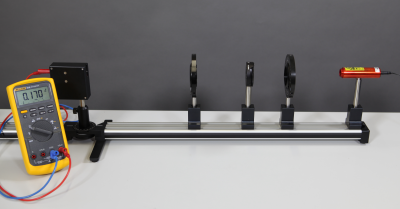
\includegraphics[width=\textwidth]{bilder/LambdaHalbe.png}
			\caption{Aufbau des zweiten Teilversuches.\cite{WWU}}
			\label{fig:LambdaHalbe}	
		\end{figure}
		Der Aufbau des zweiten Teilversuches ist in Abb. \ref{fig:LambdaHalbe} dargestellt.
		Dieser Teilversuch verläuft analog zu dem ersten, nur dass hier zusätzlich das $\lambda/2$-Plättchen zwischen den beiden Polarisatoren platziert wird.
		
		Beim Eintritt in das Plättchen sind der parallele und der orthogonale Teil des E-Feld Vektors in Phase. 
		Nach dem Durchlaufen des doppelbrechenden Plättchens ($n_1 , n_2$) ist aufgrund der unterschiedlichen Laufzeiten der beiden Komponenten eine Phasendifferenz $\Delta\phi$ zwischen ihnen entstanden.
		
		Gilt für die Dicke $d$ des Plättchens $d\cdot(n_2-n_1)=\lambda/2$, so wird $\Delta\phi=\pi$ und der E-Feld Vektor dreht sich um den Winkel $\Delta\alpha = 2\phi$.
		Drehen des $\lambda/2$-Plättchens um einen Winkel $\phi$ führt zu einer Drehung der Polarisationsebene um den doppelten Winkel $2\phi$.
		
		Für diesen Versuch soll das $\lambda/2$-Plättchen gedreht werden und beobachtet werden um welchen Winkel sich das Maximum über Drehung des zweiten Polarisators verschoben hat.
		
	\subsubsection*{Durchführung}
	
		Wie auch bei dem ersten Teilversuch war die gemessene Spannung für die Polarisatoren bei $\phi_{\text{p1}} = \SI{106+-0,4}{\degree}$ maximal.
		Zunächst wurde gesucht, bei welchem Winkel des $\lambda/2$-Plättchens das Maximum bei dem hinteren Polarisator gleich bleibt.
		Dies war bei $\phi_{0,\lambda/2} = \SI{108+-0,8}{\degree}$ der Fall.
		Zur Überprüfung, ob sich der Polarisatorwinkel für das Maximum um das Doppelte des Drehwinkels $\phi_{\lambda/2}$ verschiebt, wurde letzterer auf \SI{152+-0,8}{\degree} gesetzt.
		Daraufhin ließ sich das Maximum an dem zweiten Polarisator bei $\phi_{\text{p2}} = \SI{196+-0,4}{\degree}$ finden.
		Für $\Delta\phi_{\lambda/2} = \SI{44}{\degree}$ ($\approx \SI{45}{\degree}$ in seiner Unsicherheit) findet an dem Polarisator eine Änderung von $\Delta\phi_{\text{p2}} = \SI{90}{\degree}$ statt.
		Ausgehend von dem ursprünglichen Maximum wurden nun für fünf weitere Winkel $\phi_{\lambda/2}$ in \SI{10}{\degree} Schritten die Maximawinkel $\phi_\text{p2}$ aufgezeichnet.
	
	\subsubsection*{Datenanalyse}
		
		\begin{figure}[ht]
			\centering
			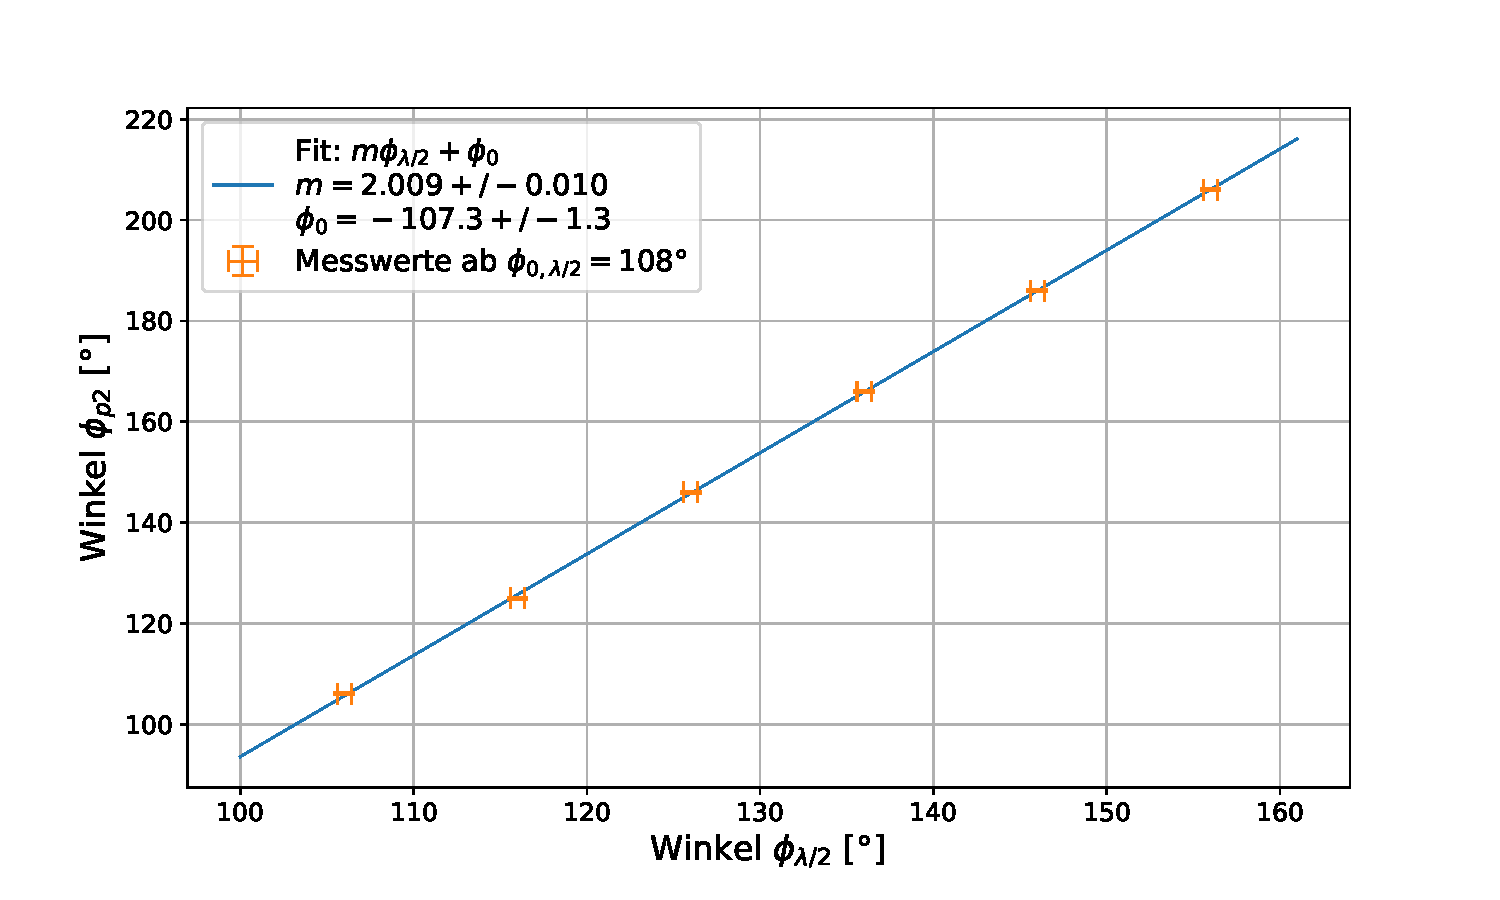
\includegraphics[width=\textwidth]{data/lambdaPolarisation.pdf}
			\caption{Messpunkte und linearer Fit für das Verhältnis $m$ der Winkel $\phi_{\lambda/2}$ und $\phi_{p2}=\phi'$.}
			\label{fig:LambdaHalbeFit}	
		\end{figure}
		Aus den Messpunkten ließ sich das Verhältnis der beiden Winkel $\phi_{\lambda/2}$ und $\phi_{p2}$ genauer bestimmen.
		Da der lineare Faktor zwei zu erwarten war, wurde an dieser Stelle ein linearer Fit verwendet.
		Abb. \ref{fig:LambdaHalbeFit} stellt diesen Verlauf und die Messpunkte dar.
		Die Steigung des Fits beträgt $m = \SI{1,998+-0,006}{}$, 2 liegt somit innerhalb einer Unsicherheit.
	
	\subsubsection*{Diskussion}
	
		Das Ergebnis dieses Teilversuches ist, dass das Verhältnis zwischen den Winkeln $\phi_{\lambda/2}$ und $\phi_{p2}$ gerade \SI{1,998+-0,006}{} entspricht.
		Der Wert ist in Übereinstimmung mit der Hypothese, dass dieses Verhältnis zwei entspricht, da er sich innerhalb der Unsicherheiten des Ergebnisses befindet.
		